\chapter{Analytical Results about the SPM}

We now have a model, the SPM, which should represent the kind of behaviour we are interested in. In this chapter we will attempt to derive analytic results about how material flows in the model. Initially this was all done with the aim of
producing an approximation to the behaviour in the hydrodynamic limit and thus informing us about the surface layer formation; however, as you will see the analytic predictions suggest that the flows could be quite interesting in their own
right.

\section{Solving Problems in Nonequlibrium Statistical Mechanics}
Models in nonequlibrium statistical mechanics which contain nontrivial interactions between components often produce interesting behaviour, hence the wide interest in these models. However, they usually prove to be difficult to ``solve'' in any
concrete sense. In this section I will give a brief overview of solution methods in equilibrium statistical mechanics, why nonequilibrium statistical mechanics problems tend to be harder to solve, and how this affects the way we approach
the SPM.


\subsection{Equilibrium Statistical Mechanics}

Equilibrium statistical mechanics is a bread and butter part of undergraduate physics, and there are a great many texts on the subject~\cite{landauLifshitzStatmech}. %others too probably, like whatever
When we speak of ``solving'' an equilibrium statistical mechanics system, the gold standard is to be able to calculate relationships between the statistics of large-scale quantities as a function of the system constraints or their conjugates.
This allows one to classify the system's behaviour by making equations of state  and identifying phase transitions  (situations where at least some large-scale quantity statistics vary with respect to each other in a discontinuous manner).
As you will see, the SPM itself is isomorphic to an equilibrium statistical mechanics model so long as we do not drive the system using boundary conditions (e.g. particle reservoirs with different concentrations).
% would like to write about the ideal gas and Ising model here
\subsubsection{Exact Solutions}

A quantity of key interest in equilibrium statistical mechanics is the partition function, usually denoted by $Z$. Say we have a closed classical mechanical system maintained at constant temperature $T$ by a heat bath,
so only energy can enter and leave the system (the canonical ensemble). Let its state space be $\Xi$, and denote an individual microstate (specific configuration of the system) by $\xi$.
Such a system must of course have a Hamiltonian $H : \Xi \rightarrow \mathbb{R}$. The canonical partition function for this system is defined to be
\begin{equation}
 Z(\beta) = \int_\Xi  \! \! \mathrm{d}  \xi \  \  e^{- \beta H(\xi)},
\end{equation}
with $\beta T = 1$, where the integrand on the right hand side is the familiar Boltzmann weighting. This quantity is extremely useful, because itself and its derivatives are directly related to the statistics of large-scale quantities.
For example, the ensemble-averaged total energy $\langle E \rangle$ satisfies
\begin{equation}
 \langle E \rangle = - \partDeriv{\log{Z}}{\beta}
\end{equation}
If one is able to obtain an expression for the canonical partition function by analytic means, you can calculate essentially any statistical moment of any large-scale quantity you desire, and thus the system is ``solved'' in the sense we used above.



\subsubsection{Approximations}


\subsection{Nonequlibrium Statistical Mechanics}

\subsubsection{Exact Solutions}

Talk about stuff like ASEP. Remember to mention that only very specific models seem to be analytically solvable, in particular you can't have interactions and range in the current models.

\subsubsection{Approximations}

Approximations in noneq statmech  

\subsubsection{Similarities and Differences Between Nonequlibrium and Equilibrium Statistical Mechanics}

\subsection{Where does the SPM stand?}
Basically, why we can't analytically solve it, and so why performing mean-field approximation is a decent start.

\section{Similarities between the SPM and Established Models in 1D}
In the previous section we have discussed the various approaches one might use when attempted to derive properties of a nonequilibrium statistical mechanical system. We will now try to put these ideas into practise on the SPM.

\subsection{Relationship with the Ising Model}

If we implement the rules of the SPM on a periodic domain, we no longer have to deal with boundary conditions. In this special circumstance, we can find an isomorphism between this model and the Ising model with fixed magnetisation.
One does this by associating the Ising spins $\sigma_i \in \left\{-1, 1 \right\}$ with $\rho_i \in \left\{ 0, 1 \right\}$ via
\begin{equation}
 \rho_i = \frac{1}{2}\left(1+\sigma_i\right).
\end{equation}
Recalling our proof that the SPM obeys detailed balance, we saw that the equilibrium probability of finding the SPM in a state containing $N$ particle-particle adjacencies is proportional to $\lambda^{-N}$.
%obviously refer to this
If our Ising Hamiltonian is defined via
\begin{equation}
 H = \frac{1}{2} \sum_{i=1}^L J \sigma_i \sigma_{i+1 \pmod L},
\end{equation}
the probability of finding ourselves in a state with $N$ paired spins is $e^{-\beta N J}$, with $\beta T =1$. The comparison with the SPM is now obvious; we set $\log{\lambda} = \beta J$. Thus $\lambda$ in the SPM is simultaneously playing the
of the binding energy and temperature in the Ising model.
!Try to compute average energy!


\subsection{Correlation Functions}
For relatively small systems, given a system size $L$ and a number of particles $N$, we can analytically compute the pairwise correlation function $C(l) = \left\langle \rho_i \rho_{i+l} \right\rangle$ (as the system is clearly homogeneous in $i$).
The following \texttt{Python} code does this:
\begin{lstlisting}[language=Python]
import copy
import sys

def configMake(L, N, prevList, totList):
    if L==1:
        endList = [copy.deepcopy(prevList), N]
        totList.append(unfold(endList))
        return [N]
    if N==0:
       return configMake(L-1, 0, [copy.deepcopy(prevList), 0], totList)
    if L==N:
        return configMake(L-1, N-1, [copy.deepcopy(prevList), 1], totList)
    return [configMake(L-1, N, [copy.deepcopy(prevList), 0], totList), configMake(L-1, N-1, [copy.deepcopy(prevList), 1], totList)]

def adjSum(candList):
    listLen = len(candList)
    total = 0
    for index in range(0, listLen):
        total += candList[index-1]*candList[index]
    return total

def unfold(candList):
    if isinstance(candList, list):
        if len(candList)==2:
            return unfold(candList[0])+unfold(candList[1])
        if len(candList)==1:
            return candList
        if len(candList)==0:
            return []
    return [candList]

def listCollate(candList):
    maxItem = 0
    for index in candList:
        if index > maxItem:
            maxItem = index
    outPut = []
    for size in range(0, maxItem+1):
        numCounts = 0
        for index in candList:
            if index == size:
                numCounts += 1
        outPut.append((size, numCounts))
    return outPut

def genCorrFn(L, N):
    totList = []
    allStates = configMake(L, N, [], totList)
    restStates = []
    weightList = []
    maxAdj = 0
    for state in totList:
        if state[0]==1:
            restStates.append((state, adjSum(state)))
            if restStates[-1][1]>maxAdj:
                maxAdj = restStates[-1][1]
            weightList.append(restStates[-1][1])
    partFnList = listCollate(weightList)
    print(partFnList)
    partitionFn = "("
    for pair in partFnList:
        partitionFn += str(pair[1])+" Exp["+str(pair[0]-maxAdj)+"b] + "
    partitionFn += "0)"
    print(partitionFn)
    finalOut = "{"
    for shift in range(0, L-L/2):
        tempList = []
        for config in restStates:
            if config[0][shift] == 1:
                tempList.append(config[1])
        stateDist = listCollate(tempList)
        outSum = "{"+str(shift)+", ("
        for pair in stateDist:
            outSum += str(pair[1])+" Exp["+str(pair[0]-maxAdj)+"b] + "
        outSum += "0)/"+partitionFn+"}"
        finalOut += outSum
        if shift != L-L/2-1:
            finalOut += ", "
    finalOut+="}"
    return finalOut

L = int(sys.argv[1])

with open("corrFnResults.m", 'w') as f:
    f.write("{")
    for n in range(2, L-2):
        f.write("{"+str(n)+"/"+str(L)+", "+genCorrFn(L, n)+"}, ")
    f.write(genCorrFn(L, L-2) + "}")
\end{lstlisting}

This is quite a nice result, as we can use simple recursion to perform a calculation which would otherwise be quite difficult to code.
Unfortunately the time complexity of the calculation grows exponentially in and $L$, so the largest $L$ I can reasonably run for is $20$. In the table below I have plotted the occupation probability of sites shifted from the origin
(assuming the origin is occupied)  for a selection of $\lambda = e^{-b}$ and particle densities.

\begin{figure}[h!]
\caption{\label{fig:corrFns} }
\begin{center}
 \begin{tabular}{c | c | c}
    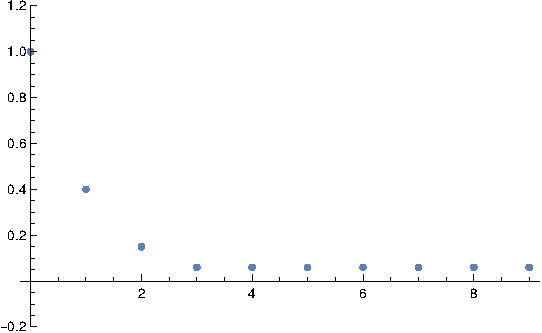
\includegraphics[width=0.32\linewidth]{analytics/images/exactCorrFns/lowDensLowL}  & 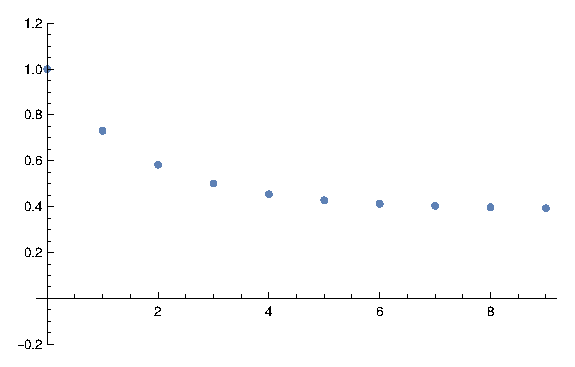
\includegraphics[width=0.32 \linewidth]{analytics/images/exactCorrFns/midDensLowL} & 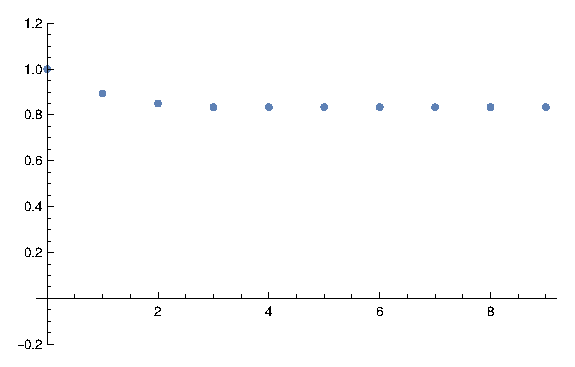
\includegraphics[width=0.32 \linewidth]{analytics/images/exactCorrFns/highDensLowL} \\
    \hline
        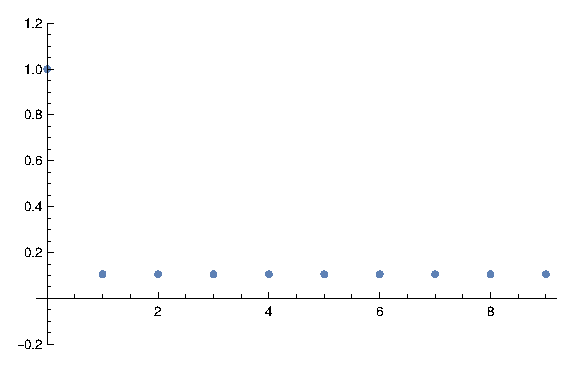
\includegraphics[width=0.32\linewidth]{analytics/images/exactCorrFns/lowDensMidL}  & 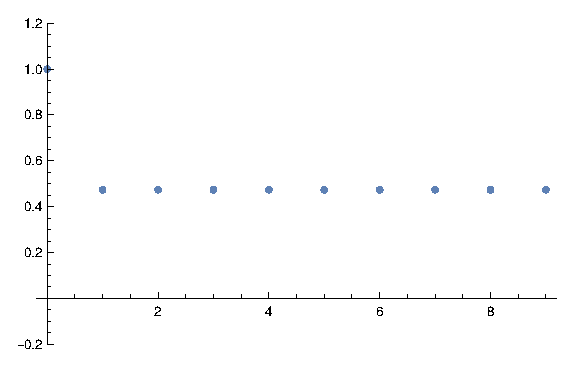
\includegraphics[width=0.32 \linewidth]{analytics/images/exactCorrFns/midDensMidL} & 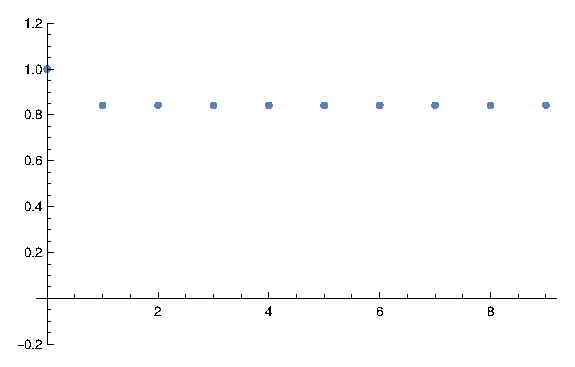
\includegraphics[width=0.32 \linewidth]{analytics/images/exactCorrFns/highDensMidL} \\
    \hline
        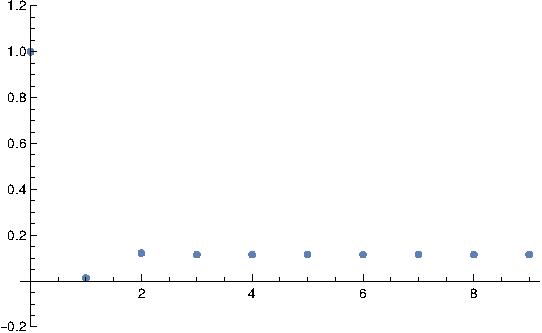
\includegraphics[width=0.32\linewidth]{analytics/images/exactCorrFns/lowDensHighL}  & 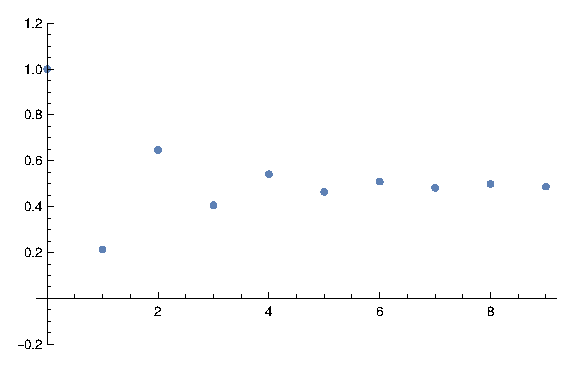
\includegraphics[width=0.32 \linewidth]{analytics/images/exactCorrFns/midDensHighL} & 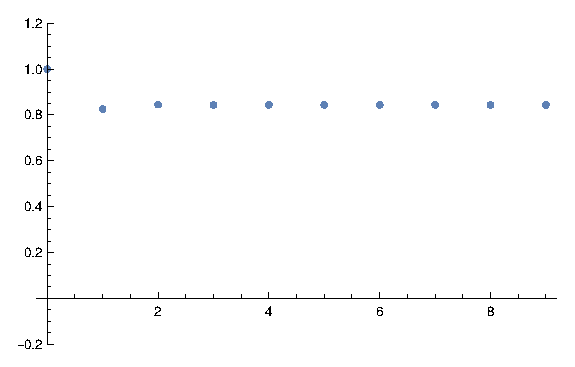
\includegraphics[width=0.32 \linewidth]{analytics/images/exactCorrFns/highDensHighL} \\
    \end{tabular}
\end{center}
    \vspace{-2em}
\end{figure}

!write some more about this sometime!

\subsection{Equivalence with the Misanthrope Process}
\begin{itemize}
 \item show the equivalence
 \item show lack of explosive condensation
 \item discuss limits of this (e.g. doesn't really clue us in to how flow works etc)
\end{itemize}

\section{Using the Mean-Field Approximation on the SPM}
\subsection{Lattice MFT Derivation}

From here we will be assuming that there isn't a way to solve the SPM exactly, so we will attempt to use approximation. MFT is, as always, and option.
\subsection{Continuum Limit MFT Derivation}
\subsection{Negative Diffusion Coefficients}
When do they happen? What do they mean?
\subsection{Continuum Limit MFT Solutions}
There's a bunch of these.
\subsection{Continuum MFT Breakdown}

\section{The SPM in Higher Dimensions}
Kinda repeat the earlier stuff in higher dimensions, particularly 2 where we actually have data. Maybe less need for elaborate sections structure here; just write freely and see how it goes.

